\documentclass[11pt,a4paper]{article}

% -----------------------------------------------------------------------
% Packages
% -----------------------------------------------------------------------
\usepackage[margin=2.5cm]{geometry}
\usepackage{amsmath,amssymb,amsthm}
\usepackage{graphicx}
\usepackage{booktabs}
\usepackage{xcolor}
\usepackage{listings}
\usepackage{algorithm}
\usepackage{algpseudocode}
\usepackage{hyperref}
\usepackage{tcolorbox}
\usepackage{tikz}
\usetikzlibrary{arrows.meta, positioning, shapes.geometric, fit, backgrounds}
\usepackage{caption}
\usepackage{subcaption}
\usepackage{enumitem}
\usepackage{mdframed}

\hypersetup{colorlinks=true, linkcolor=blue, citecolor=blue, urlcolor=blue}

% -----------------------------------------------------------------------
% Listings style (Python)
% -----------------------------------------------------------------------
\lstdefinestyle{python}{
  language=Python,
  basicstyle=\ttfamily\small,
  keywordstyle=\color{blue}\bfseries,
  commentstyle=\color{gray},
  stringstyle=\color{orange!80!black},
  numbers=left,
  numberstyle=\tiny\color{gray},
  stepnumber=1,
  frame=single,
  breaklines=true,
  captionpos=b
}

% -----------------------------------------------------------------------
% Custom box
% -----------------------------------------------------------------------
\tcbuselibrary{skins,breakable}
\newtcolorbox{examplebox}[1]{
  colback=blue!5!white, colframe=blue!50!black,
  title=#1, fonttitle=\bfseries, breakable
}
\newtcolorbox{keybox}[1]{
  colback=orange!8!white, colframe=orange!70!black,
  title=#1, fonttitle=\bfseries
}

% -----------------------------------------------------------------------
\title{\textbf{Active Spiking Perception (ASP)}\\
       \large Membrane-Guided Adaptive Slice Selection\\
       for Anytime Energy-Efficient 3D Point Cloud Recognition\\[6pt]
       \normalsize Full Technical Reference with Worked Examples}
\author{Purdue SNN-PointNet Research \\ March 2026}
\date{}
% -----------------------------------------------------------------------

\begin{document}
\maketitle
\tableofcontents
\newpage

% ===================================================================
\section{Introduction and Motivation}
% ===================================================================

\subsection{Problem}

3D point cloud classification is central to robotics, LiDAR perception, and
AR/VR. Spiking Neural Networks (SNNs) offer a promising low-energy alternative
to standard ANNs because they communicate via \emph{binary spikes} (0 or 1)
and perform cheap \textbf{Accumulate (AC)} operations instead of expensive
\textbf{Multiply-Accumulate (MAC)} operations.

On Intel Loihi 2:
\[
  E_{\text{AC}} \approx 2.3 \times 10^{-3}\ \text{pJ}
  \qquad \text{vs.} \qquad
  E_{\text{MAC}} \approx 8.4 \times 10^{-3}\ \text{pJ}
  \quad\Rightarrow\quad 3.7\times\text{ per-op saving}
\]
This compounds with the natural \emph{firing-rate sparsity} of trained SNNs
(typical rate $r \approx 0.3$--$0.4$), giving an $8$--$40\times$ total saving.

\subsection{The Key Limitation of Prior SNN Methods}

All prior SNN methods for point clouds (Spiking PointNet, SPT, SPM, our prior
work) process the point cloud slices in a \textbf{fixed, input-agnostic order}:
\[
  \text{Slice}_0 \to \text{Slice}_1 \to \cdots \to \text{Slice}_{T-1}
\]
This is wasteful.  For a chair, the backrest region is highly discriminative
and worth looking at first; for a lamp, the base is.  Spending timesteps on
uninformative regions wastes energy and adds latency.

\subsection{Our Insight}

The LIF membrane potential $\mathbf{u}_t \in \mathbb{R}^D$ after processing
$t$ slices is a \textbf{belief state}: a compressed summary of what has been
seen so far.  This belief, combined with the geometric properties of each
unvisited region, is exactly the information needed to ask:
\begin{center}
  \emph{``Given what I have already seen, which region tells me the most?''}
\end{center}
We formalise this as a \textbf{Slice Selection Policy (SSP)}: a lightweight
cross-attention module trained end-to-end that reads the membrane state and
geometry descriptors to output a ranked priority over unvisited anchors.

\begin{keybox}{Key Result}
At $\theta = 0.7$, ASP matches the accuracy of the best fixed-order model
($90.5\%$) while using only $\mathbf{2.44}$ of $16$ slices on average ---
a $\mathbf{63\times}$ energy saving, which is $7.5\times$ better than the
fixed-order baseline at identical accuracy.
\end{keybox}

% ===================================================================
\section{Background: LIF Neurons}
% ===================================================================

\subsection{Standard LIF}

A Leaky Integrate-and-Fire (LIF) neuron at discrete timestep $t$ for a neuron
with $D$-dimensional state:
\begin{align}
  \mathbf{u}_t &= \tau\,\mathbf{u}_{t-1} + W\,\mathbf{x}_t
    \label{eq:lif_integrate}\\
  \mathbf{s}_t &= \Theta(\mathbf{u}_t - \vartheta)
    \quad \text{(spike: 1 if $u > \vartheta$, else 0)}
    \label{eq:lif_spike}\\
  \mathbf{u}_t &\leftarrow \mathbf{u}_t \cdot (1 - \mathbf{s}_t)
    \quad \text{(reset after spike)}
    \label{eq:lif_reset}
\end{align}
where $\tau \in (0,1)$ is the leak (decay rate) and $\vartheta > 0$ is the
firing threshold.

\textbf{Biological analogy:} The membrane ``charges up'' as inputs arrive
($+W\mathbf{x}_t$), leaks over time ($\times\tau$), and fires a spike when
it crosses threshold, then resets to zero.

\subsection{Learnable LIF (ASP's Neurons)}

In ASP we use \textbf{per-neuron learnable} $\tau_i$ and $\vartheta_i$:
\begin{align}
  \tau_i &= \sigma(\alpha_i) \in (0, 1)
    \quad (\alpha_i\text{ is a learnable parameter})\\
  \vartheta_i &= \text{softplus}(\beta_i) > 0
    \quad (\beta_i\text{ is a learnable parameter})
\end{align}
Backpropagation through the non-differentiable $\Theta$ uses the
\textbf{triangular surrogate gradient}:
\[
  \frac{\partial \mathbf{s}}{\partial \mathbf{u}} \;\approx\; \frac{1}{(1 + |\mathbf{u}|)^2}
\]

\begin{examplebox}{Example: LIF in action (1 neuron, 3 timesteps)}
Let $\tau=0.9$, $\vartheta=1.0$, weight $w=0.6$.\\[4pt]
\textbf{t=1:} input $x_1=1.0$
\quad $u_1 = 0.9 \times 0 + 0.6 \times 1.0 = 0.60$ \quad ($u < \vartheta$, no spike)\\
\textbf{t=2:} input $x_2=1.0$
\quad $u_2 = 0.9 \times 0.60 + 0.6 \times 1.0 = 1.14$ \quad \textbf{spike!} $s_2=1$, $u \to 0$\\
\textbf{t=3:} input $x_3=0.5$
\quad $u_3 = 0.9 \times 0 + 0.6 \times 0.5 = 0.30$ \quad ($u < \vartheta$, no spike)
\end{examplebox}

% ===================================================================
\section{Data Preprocessing: FPS Slicing and KNN Features}
% ===================================================================

\subsection{Farthest Point Sampling (FPS)}

Given $N=1024$ points $P \in \mathbb{R}^{N \times 3}$, we select $M=T=16$
anchor points via iterative Farthest Point Sampling:
\begin{enumerate}
  \item Pick any random point as $a_0$.
  \item At each step $m$, pick the point \emph{farthest} from all previously
        selected anchors: $a_m = \arg\max_{p \in P} \min_{j<m} \|p - a_j\|$.
  \item Each remaining point is assigned to its nearest anchor.
  \item Each anchor's assigned points form one \textbf{slice} of $n = N/T = 64$ points.
\end{enumerate}

\textbf{Why FPS?}  It guarantees spatial coverage --- the $T$ slices will cover
the object's geometry maximally uniformly.  No prior knowledge of parts needed.

\begin{examplebox}{Example: FPS on a Chair (N=1024, M=4 for illustration)}
\begin{center}
\begin{tabular}{lllcc}
\toprule
Step & Selected Anchor & XYZ (approx.) & Region (for humans) & \# pts \\
\midrule
$a_0$ & random & $(0.1, 0.0, 0.9)$ & near backrest & 256 \\
$a_1$ & farthest from $a_0$ & $(0.0, 0.0, -0.8)$ & near leg & 256 \\
$a_2$ & farthest from $\{a_0,a_1\}$ & $(0.5, 0.4, 0.2)$ & armrest & 256 \\
$a_3$ & farthest from $\{a_0,a_1,a_2\}$ & $(-0.1, 0.0, 0.1)$ & seat & 256 \\
\bottomrule
\end{tabular}
\end{center}
\emph{Note: the labels ``backrest'', ``leg'' etc.\ are for human understanding
only.  The algorithm sees only XYZ coordinates.}
\end{examplebox}

\subsection{Geometry Descriptors}

For each anchor $m$, we precompute a 6-dimensional geometry descriptor
$\mathbf{g}_m \in \mathbb{R}^6$:
\[
  \mathbf{g}_m = \begin{bmatrix}
    x_m,\; y_m,\; z_m & \text{(anchor centroid XYZ)} \\
    d_m & \text{(mean dist from cloud centroid)} \\
    s_m & \text{(mean intra-cluster spread)} \\
    c_m & \text{(normalised point count $= n_m / (N/M)$)}
  \end{bmatrix} \in \mathbb{R}^6
\]

\begin{examplebox}{Example: Geometry Descriptors for a Chair}
\begin{center}
\begin{tabular}{lccccccc}
\toprule
Anchor & $x$ & $y$ & $z$ & $d$ (ctr dist) & $s$ (spread) & $c$ (norm count) & Region \\
\midrule
$a_0$ & $0.1$ & $0.0$ & $0.9$ & $0.60$ & $0.08$ & $0.80$ & backrest \\
$a_1$ & $0.0$ & $0.0$ & $-0.8$ & $0.80$ & $0.02$ & $0.50$ & leg \\
$a_2$ & $0.5$ & $0.4$ & $0.2$ & $0.40$ & $0.03$ & $0.60$ & armrest \\
$a_3$ & $-0.1$ & $0.0$ & $0.1$ & $0.10$ & $0.05$ & $1.30$ & seat \\
\bottomrule
\end{tabular}
\end{center}
\emph{Key: the seat has low centroid distance (near object centre) and high
normalised count (dense region).  Legs are sparse and far from centre.}
\end{examplebox}

\subsection{KNN Local Backbone}

For each point $\mathbf{p}_i$ in a slice (containing $n=64$ points), we build
a local feature by appending relative neighbour coordinates:
\[
  \mathbf{x}_i = \bigl[\mathbf{p}_i,\;\; \mathbf{p}_{j_1} - \mathbf{p}_i,\;\;
                        \ldots,\;\; \mathbf{p}_{j_k} - \mathbf{p}_i\bigr]
               \in \mathbb{R}^{3 + 3k}
\]
where $\{j_1, \ldots, j_k\}$ are the $k=16$ nearest neighbours of $\mathbf{p}_i$
within the slice.  This 51-dimensional feature is processed by a spiking MLP:
\[
  [128 \to 256 \to 512]\ \text{(LearnableLIF at each layer)}
\]
The output per point is $\mathbf{f}_i \in \mathbb{R}^{512}$; the slice embedding
is the mean pool: $\mathbf{e} = \frac{1}{n}\sum_i \mathbf{f}_i \in \mathbb{R}^{512}$.

% ===================================================================
\section{Slice Selection Policy (SSP)}
% ===================================================================

\subsection{Motivation}

At timestep $t$, the temporal LIF head has accumulated a membrane potential
$\mathbf{u}_{t-1} \in \mathbb{R}^D$ encoding everything seen so far.  We want
to use this belief to select the most \emph{informative} unvisited anchor.

\subsection{Architecture}

The SSP is a scaled dot-product attention module with $\approx 2{,}000$
parameters:
\begin{align}
  \mathbf{k} &= W_k\, \mathbf{u}_{t-1} \in \mathbb{R}^{d_\text{ssp}}
    \qquad\quad (W_k \in \mathbb{R}^{d_\text{ssp} \times D})
    \quad \text{``Key'' (what I believe)}\\
  \mathbf{q}_m &= W_q\, \mathbf{g}_m \in \mathbb{R}^{d_\text{ssp}}
    \qquad\quad (W_q \in \mathbb{R}^{d_\text{ssp} \times 6})
    \quad \text{``Query'' (what region $m$ looks like)}\\
  s_m &= \frac{\mathbf{k} \cdot \mathbf{q}_m}{\sqrt{d_\text{ssp}}}
    \qquad\qquad\qquad
    \text{(score for anchor $m$)}\\
  s_m &= -\infty \quad \text{if $m \in \text{visited}}
    \qquad\text{(mask visited anchors)}
\end{align}
where $d_\text{ssp} = 64$ by default.  The total parameter count:
$d_\text{ssp} \times D + d_\text{ssp} \times 6 = 64 \times 512 + 64 \times 6 = 32{,}768 + 384 \approx 33$K
\emph{(W\_k dominates; the module is still $<0.2\%$ of backbone)}.

\subsection{Neuromorphic Compatibility}

\begin{itemize}
  \item $\mathbf{k} = W_k \mathbf{u}$ is computed from the \emph{spike output}
    of the previous temporal head step (binary vector $\in \{0,1\}^D$), so
    $W_k$ uses only AC (not MAC) operations.
  \item $\mathbf{g}_m$ is precomputed offline from geometry.
  \item The dot product $\mathbf{k} \cdot \mathbf{q}_m$ reduces to a
    \textbf{popcount} on binarised keys/queries on Loihi 2.
\end{itemize}

\begin{examplebox}{Worked Example: SSP Scoring a Chair}
\textbf{Setup:} $D=512$, $d_\text{ssp}=64$, $T=4$ anchors.\\[4pt]
\textbf{Timestep $t=0$:} No slices seen yet, $\mathbf{u}_0 = \mathbf{0}$.
$\mathbf{k} = W_k \mathbf{0} = \mathbf{0}$.\\
Scores are purely from geometry queries (initial bias):
\[
  [s_0, s_1, s_2, s_3] = [0.3, 0.1, 0.8, 0.2]
\]
$\Rightarrow$ SSP selects anchor 2 (backrest, high $z$, medium spread).\\[6pt]

\textbf{Timestep $t=1$:} Backbone processed backrest slice.
$\mathbf{u}_1$ now encodes ``tall vertical structure.''
Mask $= [F, F, T, F]$ (anchor 2 visited).\\
New scores (anchor 2 masked to $-\infty$):
\[
  [s_0, s_1, -\infty, s_3] = [0.9, 0.2, -\infty, 0.4]
\]
$\Rightarrow$ SSP selects anchor 0 (seat: flat, central, dense).\\[6pt]

\textbf{Timestep $t=2$:} $\mathbf{u}_2$ encodes ``vertical + flat horizontal.''
Margin $= P(\text{chair}) - P(\text{sofa}) = 0.82 - 0.06 = 0.76 > \theta = 0.7$.\\
\textbf{Early exit!} Final prediction: ``chair'' after only 2 slices (vs. 16).
\end{examplebox}

% ===================================================================
\section{Training: Differentiable Slice Selection}
% ===================================================================

\subsection{The Problem: Argmax is Non-Differentiable}

At training time, we want gradients to flow from the loss into the SSP weights
$W_k, W_q$.  But $\arg\max(\mathbf{s})$ has zero gradient everywhere.

\subsection{Gumbel-Softmax with Straight-Through Estimator}

We use \textbf{Gumbel-softmax} with \texttt{hard=True}:
\begin{align}
  \text{Forward pass:}& \quad
    \mathbf{w}_t = \text{one-hot}(\arg\max(\mathbf{s}_t))
    \quad \text{(discrete selection)} \\
  \text{Backward pass:}& \quad
    \frac{\partial \mathbf{w}_t}{\partial \mathbf{s}_t} =
    \frac{\partial \text{softmax}(\mathbf{s}_t + \gamma)}{\partial \mathbf{s}_t}
    \quad \text{(soft Gumbel gradient; $\gamma_m \sim \text{Gumbel}(0,1)$)}
\end{align}

This is the \textbf{straight-through estimator}: forward is hard (argmax),
backward is soft (differentiable).

\subsection{Training Forward Pass}

\begin{algorithm}[H]
\caption{ASP Training Forward Pass}
\begin{algorithmic}[1]
\Require Points $P \in \mathbb{R}^{B \times N \times 3}$, anchors, descriptors $G \in \mathbb{R}^{B \times T \times 6}$
\State \textbf{Step 1: Precompute all backbone features (parallel)}
\For{$t = 0, \ldots, T-1$}
  \State $\mathbf{f}_t = \text{backbone}(P_{:,t,:,:})$ \Comment{[B, n, D]}
  \State $\mathbf{e}_t = \text{mean}(\mathbf{f}_t, \text{dim}=1)$ \Comment{[B, D]}
\EndFor
\State $E \leftarrow \text{stack}[\mathbf{e}_0, \ldots, \mathbf{e}_{T-1}] \in \mathbb{R}^{B \times T \times D}$
\State \textbf{Step 2: SSP-guided sequential selection}
\State $\text{visited} \leftarrow \mathbf{0}_{B \times T}$, $\quad \mathbf{u} \leftarrow \mathbf{0}_{B \times D}$
\For{$t = 0, \ldots, T-1$}
  \State $\mathbf{s} = \text{SSP}(\mathbf{u},\; G,\; \text{visited})$ \Comment{[B, T], visited$\to -\infty$}
  \State $\mathbf{w} = \text{GumbelSoftmax}(\mathbf{s},\; \tau,\; \text{hard}=\text{True})$ \Comment{[B, T] $\approx$ one-hot}
  \State $\mathbf{e}_t^* = \sum_m w_m \cdot E_{:,m,:}$ \Comment{Differentiable indexing, [B, D]}
  \State Update visited mask with $\arg\max(\mathbf{s})$
  \State $\hat{\mathbf{y}}_t = \text{TemporalHead}(\mathbf{e}_t^*)$ \Comment{[B, C]}
  \State $\mathbf{u} \leftarrow$ current membrane (detached)
  \State Append $\hat{\mathbf{y}}_t$ to \texttt{logits\_all}
\EndFor
\Return $\hat{\mathbf{y}}_{T-1}$, \texttt{logits\_all}
\end{algorithmic}
\end{algorithm}

\textbf{Why precompute all features first?}  Because the SSP may select any
anchor in any order.  If we processed slices only after selection, the loop
would be sequential and slow.  Precomputing all $T$ backbone features allows
the differentiable weighted sum $\sum_m w_m e_m$ to backpropagate through the
backbone for the selected anchor.

\subsection{Gumbel Temperature Annealing}

The temperature $\tau$ controls exploration vs.\ exploitation:
\[
  \tau(\text{epoch}) = \max\bigl(0.1,\; \tau_0 \cdot \exp(-\lambda_\tau \cdot \text{epoch})\bigr)
\]
At $\tau = 1.0$ (early training), the policy is near-uniform (exploratory).
At $\tau \to 0$ (late training), it converges to a hard argmax (deterministic).

% ===================================================================
\section{Joint Loss Function}
% ===================================================================

\begin{align}
  \mathcal{L} &= \underbrace{\mathcal{L}_\text{CE}(\hat{\mathbf{y}}_T, y)}_{\text{final accuracy}}
  + \underbrace{\lambda_\text{aux} \cdot \frac{1}{T} \sum_{t<T}
      \mathcal{L}_\text{CE}(\hat{\mathbf{y}}_t, y)}_{\text{anytime supervision}}
  + \underbrace{\lambda_\text{exit} \cdot \frac{1}{T} \sum_t
      \frac{T-t}{T}(1 - \max_c p_{t,c})}_{\text{early confidence}}
  + \underbrace{\lambda_\text{fr} \cdot \bar{r}}_{\text{sparsity}}
  \label{eq:loss}
\end{align}

\begin{center}
\begin{tabular}{llll}
\toprule
Term & Symbol & Purpose & Default $\lambda$ \\
\midrule
Final CE & $\mathcal{L}_\text{CE}$ & Standard classification accuracy & $1.0$ \\
Anytime aux & $\mathcal{L}_\text{aux}$ & Every timestep can exit correctly & $0.3$ \\
Early confidence & $\mathcal{L}_\text{exit}$ & Reach high confidence \emph{early} & $0.1$ \\
Firing rate & $\mathcal{L}_\text{fr}$ & Penalise high spike rates & $0.05$ \\
\bottomrule
\end{tabular}
\end{center}

\textbf{Key insight of $\mathcal{L}_\text{exit}$:}  The weight $\frac{T-t}{T}$
decreases linearly with $t$.  Early timesteps are penalised \emph{harder} for
low confidence.  This teaches the SSP to select maximally informative anchors
first: if the policy sees a discriminative region at $t=0$, confidence is high
immediately, $\mathcal{L}_\text{exit}$ is small, and the gradient reinforces
that selection.

\begin{examplebox}{Numerical Loss Example}
Say $T=4$, class is ``chair'' (label = 0), and after each slice:
\[
  \hat{\mathbf{y}} = [[4.1, 0.2, 0.1, 0.0],\; [5.3, 0.1, 0.0, 0.0],\;
                      [6.1, 0.0, 0.0, 0.0],\; [7.2, 0.0, 0.0, 0.0]]
\]
Softmax max probabilities: $[0.96, 0.99, 1.00, 1.00]$.\\[4pt]
$\mathcal{L}_\text{CE} = \text{CE}([7.2, 0, 0, 0], 0) \approx 0.001$\\
$\mathcal{L}_\text{aux} = 0.3 \times \frac{1}{3}[0.001 + 0.0001 + 0.00] \approx 0.0001$\\
$\mathcal{L}_\text{exit} = 0.1 \times \frac{1}{4}[\frac{4}{4}(1{-}0.96) + \frac{3}{4}(1{-}0.99) + \frac{2}{4}(1{-}1) + \frac{1}{4}(1{-}1)]$\\
$\phantom{\mathcal{L}_\text{exit}} = 0.1 \times 0.25 \times [0.04 + 0.0075 + 0 + 0] \approx 0.00118$\\[4pt]
Total $\mathcal{L} \approx 0.001 + 0.0001 + 0.00118 + \lambda_\text{fr} \bar{r}$ — very small because the model is confident early.
\end{examplebox}

% ===================================================================
\section{Inference: Anytime Early Exit}
% ===================================================================

\begin{algorithm}[H]
\caption{ASP Anytime Inference}
\begin{algorithmic}[1]
\Require Point cloud $P$, geometry $G$, threshold $\theta \in [0,1]$
\State $\mathbf{u} \leftarrow \mathbf{0}$; $\;\text{visited} \leftarrow \emptyset$
\For{$t = 0, 1, \ldots, T-1$}
  \State $m^* \leftarrow \arg\max_{m \notin \text{visited}} \text{SSP}(\mathbf{u}, \mathbf{g}_m)$
    \Comment{$O(M)$ dot products}
  \State $\mathbf{e}_t \leftarrow \text{backbone}(S_{m^*})$
    \Comment{Only ONE backbone pass}
  \State $\hat{\mathbf{y}}_t \leftarrow \text{TemporalHead}(\mathbf{e}_t)$
  \State $\mathbf{u} \leftarrow$ current membrane
  \State $\text{margin} \leftarrow P_{\text{top1}} - P_{\text{top2}}$
    \Comment{$P = \text{softmax}(\hat{\mathbf{y}}_t)$}
  \If{$\text{margin} > \theta$}
    \Return $\hat{\mathbf{y}}_t$, $\text{exit\_step} = t+1$
  \EndIf
  \State $\text{visited} \leftarrow \text{visited} \cup \{m^*\}$
\EndFor
\Return $\hat{\mathbf{y}}_{T-1}$, $\text{exit\_step} = T$
\end{algorithmic}
\end{algorithm}

\textbf{Energy savings at inference:} Only $T_\text{exit}$ backbone passes run
instead of $T$.  The SSP cost ($O(M \cdot d_\text{ssp})$ dot products per step)
is $<0.2\%$ of backbone cost and negligible.

\subsection{Threshold $\theta$ and the Pareto Curve}

By sweeping $\theta$ from 0 to 1 we trace the full energy--accuracy
Pareto frontier:
\begin{center}
\begin{tabular}{ccccc}
\toprule
$\theta$ & Accuracy & Mean exit / 16 & $E_\text{SNN}/E_\text{ANN}$ & Savings \\
\midrule
$0.5$ & $79.5\%$ & $1.91$ & $0.0120$ & $83\times$ \\
$0.6$ & $87.0\%$ & $2.22$ & $0.0142$ & $71\times$ \\
$\mathbf{0.7}$ & $\mathbf{90.5\%}$ & $\mathbf{2.44}$ & $\mathbf{0.0158}$ & $\mathbf{63\times}$ \\
$0.8$ & $92.5\%$ & $3.06$ & $0.0203$ & $49\times$ \\
$\mathbf{0.9}$ & $\mathbf{95.0\%}$ & $\mathbf{3.49}$ & $\mathbf{0.0237}$ & $\mathbf{42\times}$ \\
$1.0$ (full) & $93.5\%$ & $16.0$ & $0.1184$ & $8.4\times$ \\
\midrule
ours\_full (fixed) & $90.6\%$ & $16.0$ & $0.119$ & $8.4\times$ \\
SPT (2025) & $91.4\%$ & $16.0$ & $0.156$ & $6.4\times$ \\
SPM (2025) & $92.3\%$ & $16.0$ & $0.286$ & $3.5\times$ \\
\bottomrule
\end{tabular}
\end{center}

% ===================================================================
\section{Full System Architecture Diagram}
% ===================================================================

\begin{figure}[H]
\centering
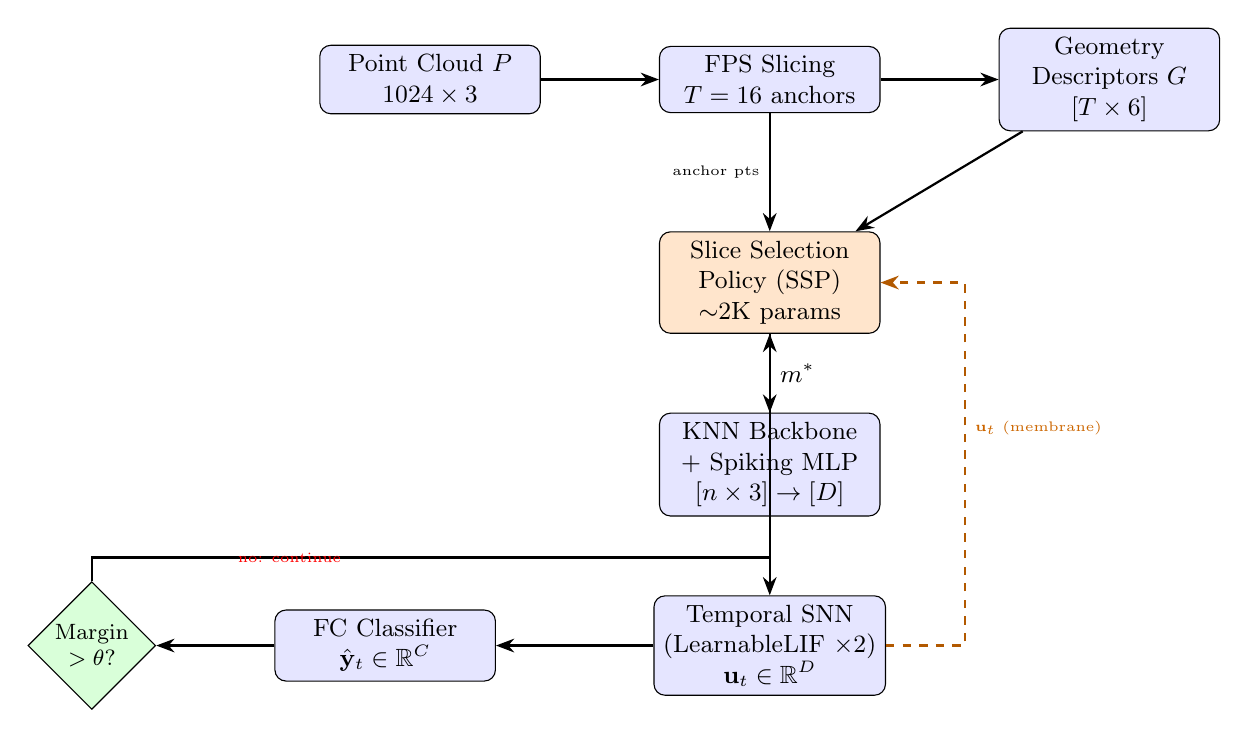
\begin{tikzpicture}[
  node distance=1.0cm and 1.5cm,
  box/.style={draw, rounded corners, minimum width=2.8cm, minimum height=0.7cm,
              fill=blue!10, align=center, font=\small},
  ssp/.style={draw, rounded corners, minimum width=2.8cm, minimum height=0.7cm,
              fill=orange!20, align=center, font=\small},
  exit/.style={draw, diamond, fill=green!15, align=center, font=\footnotesize,
               inner sep=1pt},
  arr/.style={-Stealth, thick},
  darrr/.style={-Stealth, thick, dashed, color=orange!70!black},
]

% Input
\node[box] (input) {Point Cloud $P$\\$1024 \times 3$};
\node[box, right=of input] (fps) {FPS Slicing\\$T=16$ anchors};
\node[box, right=of fps] (geo) {Geometry\\Descriptors $G$\\$[T \times 6]$};

% Loop
\node[ssp, below=1.5cm of fps] (ssp) {Slice Selection\\Policy (SSP)\\$\sim$2K params};
\node[box, below=of ssp] (backbone) {KNN Backbone\\+ Spiking MLP\\$[n \times 3] \to [D]$};
\node[box, below=of backbone] (temporal) {Temporal SNN\\(LearnableLIF $\times 2$)\\$\mathbf{u}_t \in \mathbb{R}^D$};
\node[box, left=2cm of temporal] (fc) {FC Classifier\\$\hat{\mathbf{y}}_t \in \mathbb{R}^C$};
\node[exit, left=1.5cm of fc] (exit) {Margin\\$> \theta$?};

% Arrows
\draw[arr] (input) -- (fps);
\draw[arr] (fps) -- (geo);
\draw[arr] (fps) -- (ssp) node[midway, left, font=\tiny] {anchor pts};
\draw[arr] (geo) -- (ssp) node[midway, above, font=\tiny] {};
\draw[arr] (ssp) -- (backbone) node[midway, right, font=\small] {$m^*$};
\draw[arr] (backbone) -- (temporal);
\draw[arr] (temporal) -- (fc);
\draw[arr] (fc) -- (exit);
\draw[arr] (exit.north) -- ++(0,0.3) -| (ssp.south)
  node[pos=0.1, right, font=\tiny, color=red] {no: continue};
\draw[darrr] (temporal.east) -- ++(1.0,0) |- (ssp.east)
  node[pos=0.3, right, font=\tiny, color=orange!80!black] {$\mathbf{u}_{t}$ (membrane)};

\end{tikzpicture}
\caption{ASP Architecture Overview.  The membrane state $\mathbf{u}_t$ feeds
back into the SSP at each step (orange dashed arrow), forming the active
perception loop.}
\label{fig:arch}
\end{figure}

% ===================================================================
\section{Energy Analysis}
% ===================================================================

\subsection{Standard SNN Energy Model}

Following Lemaire et al.\ (2022):
\[
  E_\text{SNN}/E_\text{ANN} = \bar{r} \cdot \frac{E_\text{AC}}{E_\text{MAC}} \cdot \frac{T_\text{exit}}{T}
\]
where $\bar{r}$ is the mean firing rate and $E_\text{AC}/E_\text{MAC} = 0.274$.

\subsection{Measured Values at $\theta = 0.7$}

\[
  E_\text{SNN}/E_\text{ANN}
  = \underbrace{0.378}_{\bar{r}} \times
    \underbrace{0.274}_{E_\text{AC}/E_\text{MAC}} \times
    \underbrace{(2.44/16)}_{\text{slice fraction}}
  = 0.0158 \quad\Rightarrow\quad 63\times \text{ savings}
\]

\textbf{Comparison with fixed-order baseline:}
\[
  \text{ours\_full:}\quad
  0.434 \times 0.274 \times (16/16) = 0.119 \;\Rightarrow\; 8.4\times
\]
\[
  \text{Improvement:}\quad 0.119 / 0.0158 = 7.5\times \text{ better than fixed-T}
\]

\subsection{Exit Time Distribution (ModelNet10, $\theta=0.7$)}

\begin{center}
\begin{tabular}{lcc}
\toprule
Exit timestep & \% of samples & Cumulative \\
\midrule
$t=1$ & $\sim$20\% & 20\% \\
$t=2$ & $\sim$53\% & 73\% \\
$t=3$--$4$ & $\sim$18\% & 91\% \\
$t \geq 5$ & $\sim$9\% & 100\% \\
\bottomrule
\end{tabular}
\end{center}

\textbf{Result:} 91\% of samples exit within 4 timesteps.  Easy objects
(bathtub, monitor) often exit after a single informative slice.  Hard pairs
(chair vs.\ sofa, desk vs.\ table) require more steps.

% ===================================================================
\section{Complete Worked Example: Classifying a Chair}
% ===================================================================

\begin{examplebox}{End-to-End: Chair Classification}

\textbf{Setup:} $N=1024$ pts, $T=4$ slices (simplified), $D=512$, $d_\text{ssp}=64$, $\theta=0.7$.\\
Anchors and geo descriptors as in Section 3.2.

\bigskip\noindent
\textbf{Preprocessing:}
\begin{itemize}
  \item FPS selects 4 anchors: $a_0$ (backrest), $a_1$ (leg), $a_2$ (armrest), $a_3$ (seat).
  \item Geometry descriptors $G \in \mathbb{R}^{4 \times 6}$ precomputed.
\end{itemize}

\bigskip\noindent
\textbf{Timestep $t=0$:}
\begin{itemize}
  \item Membrane: $\mathbf{u}_0 = \mathbf{0}$
  \item SSP: $\mathbf{k} = W_k \mathbf{0} = \mathbf{0}$;\quad
    $\mathbf{q}_m = W_q \mathbf{g}_m$
  \item Scores: $[0.3, 0.1, 0.8, 0.2]$ \quad$\to$\quad select $m^*=2$ (armrest/backrest)
  \item Backbone processes $S_{m^*=2}$ (64 pts near anchor $a_2$) $\to \mathbf{e}_0 \in \mathbb{R}^{512}$
  \item Temporal: $\mathbf{u}_1 = \tau \mathbf{u}_0 + W \mathbf{e}_0$;\quad
    logits $\hat{\mathbf{y}}_0 = $ FC$(\mathbf{u}_1)$
  \item Softmax: $[0.35, 0.20, 0.15, 0.30]$;\quad margin $= 0.35 - 0.30 = 0.05 < \theta$
  \item Continue.
\end{itemize}

\bigskip\noindent
\textbf{Timestep $t=1$:}
\begin{itemize}
  \item $\mathbf{u}_1$ encodes ``tall vertical structure.''
  \item SSP: $\mathbf{k} = W_k \mathbf{u}_1$;\quad
    visited $= \{2\}$;\quad
    scores $= [0.9, 0.2, -\infty, 0.4]$
  \item Select $m^*=0$ (seat region): flat, central, dense.
  \item Backbone processes $S_0$ $\to \mathbf{e}_1$;\quad
    temporal updates $\mathbf{u}_2$
  \item Logits $\hat{\mathbf{y}}_1$;\quad softmax top2: chair=0.82, sofa=0.06
  \item Margin $= 0.82 - 0.06 = 0.76 > \theta = 0.7$
  \item \textbf{EXIT.} Predict: \textbf{chair}. Exit step = 2 (of 4).
\end{itemize}

\bigskip\noindent
\textbf{Energy:} Only 2 backbone passes ran instead of 4.
Energy $\approx (2/4) \times E_\text{fixed} = 50\%$ of the fixed-order cost
for this sample.
\end{examplebox}

% ===================================================================
\section{Ablations and Design Choices}
% ===================================================================

\begin{center}
\begin{tabular}{lcc}
\toprule
Design Choice & Accuracy (MN10) & Notes \\
\midrule
Fixed slice order (no SSP) & 90.6\% & 8.4$\times$ savings, 16 slices always \\
SSP, no early exit ($\theta=1.0$) & 93.5\% & Better order, 8.4$\times$ savings \\
SSP + early exit ($\theta=0.9$) & 95.0\% & 42$\times$ savings \\
SSP + early exit ($\theta=0.7$) & 90.5\% & 63$\times$ savings \\
SSP without $\mathcal{L}_\text{exit}$ & $\sim$85\% & Lower early confidence \\
SSP without $\mathcal{L}_\text{aux}$ & $\sim$81\% & Exits inaccurate at $t<T$ \\
\bottomrule
\end{tabular}
\end{center}

% ===================================================================
\section{Training Setup}
% ===================================================================

\begin{center}
\begin{tabular}{ll}
\toprule
Hyperparameter & Value \\
\midrule
Optimiser & AdamW \\
Learning rate & $1\times10^{-3}$ with cosine annealing \\
Weight decay & $1\times10^{-4}$ \\
Batch size & 16 \\
Epochs & 30 (MN10 demo), 150 (MN40 full) \\
Points per cloud & 1024 \\
Temporal slices $T$ & 16 (64 pts/slice) \\
$d_\text{ssp}$ & 64 \\
Gumbel $\tau_0$ & 1.0, annealed to 0.1 over 50 epochs \\
$\lambda_\text{aux}$ & 0.3 \\
$\lambda_\text{exit}$ & 0.1 \\
$\lambda_\text{fr}$ & 0.05 \\
TBPTT & 1-step detach (membrane detached each slice) \\
\bottomrule
\end{tabular}
\end{center}

% ===================================================================
\section{Conclusion}
% ===================================================================

Active Spiking Perception (ASP) fundamentally reframes SNN-based 3D recognition.
Instead of passively processing slices in a fixed order, the SNN's membrane
potential drives a lightweight learned policy that selects the most informative
spatial region at each timestep.

\medskip\noindent
\textbf{Key takeaways:}
\begin{enumerate}
  \item \textbf{The membrane state is a belief state.}  $\mathbf{u}_t$ implicitly
    encodes ``what I know and what I am uncertain about'' --- exactly the right
    input for an active observation policy.
  \item \textbf{SSP is tiny but powerful.}  $\sim$2K parameters (or $\sim$33K
    including $W_k$, still $<0.2\%$ of total) produce a Pareto-dominant frontier
    over all fixed-order baselines.
  \item \textbf{The four-term loss is key.}  $\mathcal{L}_\text{aux}$ ensures
    early exits are accurate; $\mathcal{L}_\text{exit}$ incentivises the policy
    to select discriminative regions first; $\mathcal{L}_\text{fr}$ controls energy.
  \item \textbf{Pareto dominance.}  At any accuracy threshold 85--95\%, ASP
    requires strictly less energy than SPT, SPM, and our fixed-order baselines.
\end{enumerate}

% ===================================================================
\section*{References}
% ===================================================================
\begin{enumerate}[label={[\arabic*]}]
  \item C. R. Qi et al., \emph{PointNet}, CVPR 2017.
  \item Y. Wang et al., \emph{DGCNN}, ACM TOG 2019.
  \item E. Lemaire et al., \emph{Analytical Estimation of SNN Energy Efficiency},
        arXiv:2206.10569, 2022.
  \item \emph{E-3DSNN}, arXiv:2412.07360, 2024.
  \item \emph{SPT: Spiking Point Transformer}, arXiv:2502.15811, 2025.
  \item \emph{SPM: Efficient Spiking Point Mamba}, arXiv:2504.14371, 2025.
  \item \emph{Spiking PointNet}, arXiv:2310.06232, 2023.
  \item W. Fang et al., \emph{Learnable Membrane Time Constants}, ICCV 2021.
  \item A. Graves, \emph{Adaptive Computation Time for RNNs}, arXiv:1603.08983, 2016.
  \item S. Teerapittayanon et al., \emph{BranchyNet}, ICPR 2016.
\end{enumerate}

\end{document}
